% !TeX root = main.tex
% !TeX spellcheck = de_DE
% !TeX encoding = utf8

\chapter{Flash Memory}
Flash memory often in the form of solid state drives (SSD) are becoming more and more of primary storage for computers. The cost per storage has been decreasing steadily therefore driving adoption. Especially the low access latency and the high possible throughput compared so spinning disk hard drives are an advantage. In the application predominantly NAND type flash is used due to its higher density. 


\section{Flash Basics}
NAND flash which will be discussed is of most interest for SSDs due to its high density and therefore lower cost per bit. \cref{fg_tans} shows a floating gate transistor which is used to store data. By inserting charge into the floating gate it is possible to change the threshold voltage of the transistor. Multiple of these floating gate transistor are connected in series to for a so called NAND string. In this nand string the drain and source neighboring transistors are connected to form a continuos string as seen in \cref{nand_string}. Also on the top is a normal bit line select transistor to connect the string to be read to a bit line. On the bottom is the ground select transistor to connect the string to ground\cite[p.~22-24]{MiMa18}.

\begin{figure}
    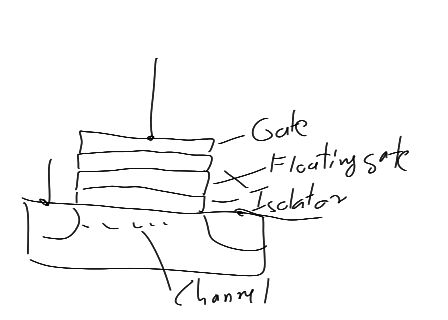
\includegraphics[width=5cm]{fg_schema.png}
    \centering
    \caption{A floating gate field effect transistor}
    \label{fg_tans}
\end{figure}


\begin{figure}
    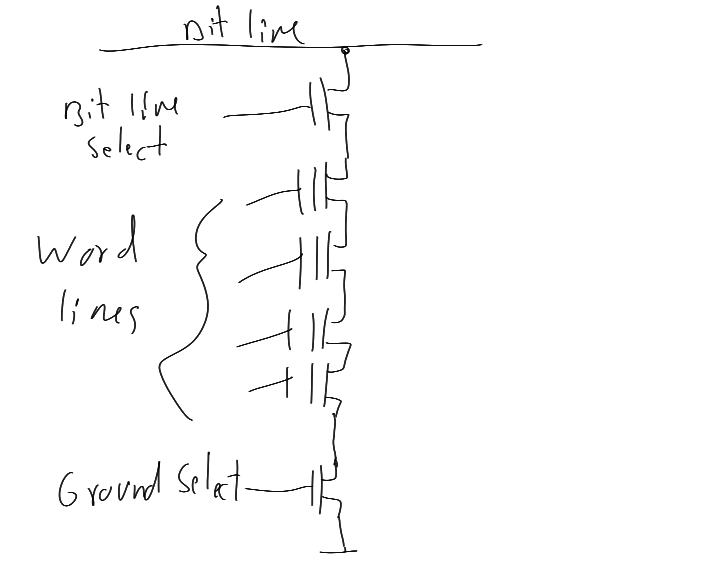
\includegraphics[width=5cm]{nand_schema.png}
    \centering
    \caption{Multiple transistors are arranged to make a NAND string}
    \label{nand_string}
\end{figure}

NAND Flash is arranged into blocks and pages. Due to its arrangement NAND memory can only be erased whole pages at a time. Whereas each block can be programmed individually. When a cell is erased, in its "0" state,  

\begin{figure}
    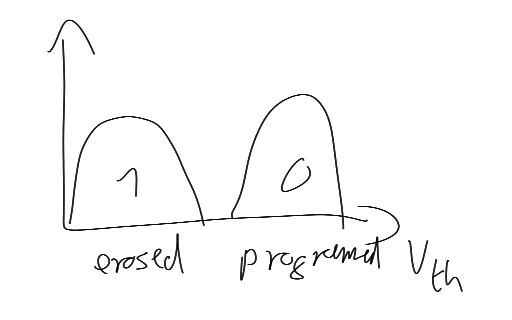
\includegraphics[width=5cm]{vth_diag.png}
    \centering
    \caption{Threshold Distribution of a Floating Gate Transistor}
    \label{nand_th}
\end{figure}

\section{Error Types}


\cite{ZaTu16}